\documentclass[usenames,dvipsnames,10pt,aspectratio=169]{beamer} 

\usepackage[utf8]{inputenc}
\usepackage{verbatim}
\usepackage{minted}
\usepackage{graphicx}
\usepackage{wrapfig}
\usepackage{geometry}
\usepackage{listings}
% \usepackage{showframe}
\usepackage{enumitem}
\usepackage{color, xcolor}
\usepackage[document]{ragged2e}
\usetheme{umu}

\usemintedstyle{monokai}

\usepackage{hyperref}
\hypersetup{
    colorlinks=true,
    linkcolor=ucugreyish,
    filecolor=ucured,
    urlcolor=ucublue,
}
\urlstyle{same}

%%% Some useful commands
% pdf-friendly newline in links
\newcommand{\pdfnewline}{\texorpdfstring{\newline}{ }} 
% Fill the vertical space in a slide (to put text at the bottom)
\newcommand{\framefill}{\vskip 0pt plus 1 filll}

%%% Enter additional packages below (or above, I can't stop you)! / Jesper
\renewcommand{\proofname}{\sffamily{Proof}}

% custom fullpage image:
% { % all template changes are local to this group.
%     \setbeamertemplate{navigation symbols}{}
%     \begin{frame}<article:0>[plain]
%         \begin{tikzpicture}[remember picture,overlay]
%             \node[at=(current page.center)] {
%                 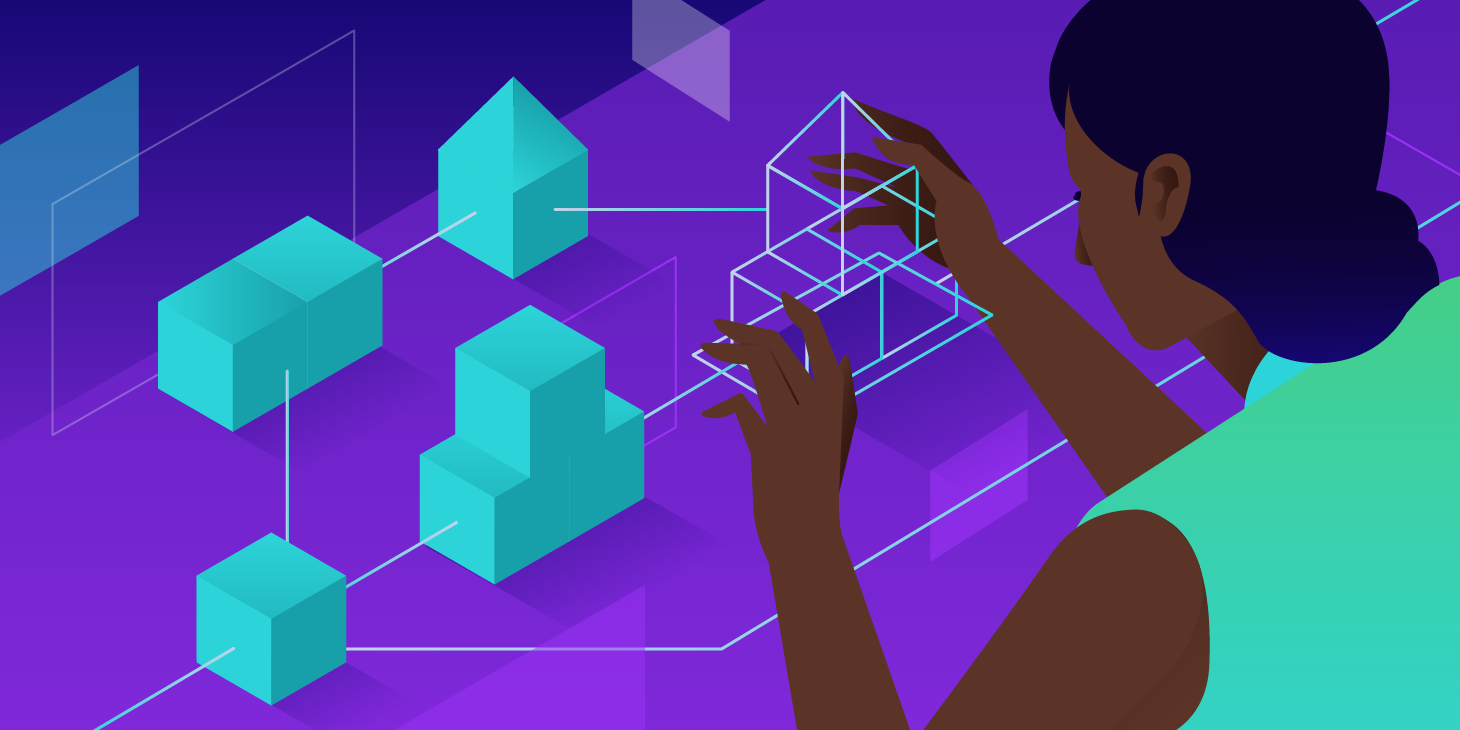
\includegraphics[width=\paperwidth,height=\paperheight]{graphics/version-control.png}
%             };
%         \end{tikzpicture}
%      \end{frame}
% }

% custom shell example inplace
% [fragile] frame
% \begin{lstlisting}[language=Bash, style=shellstyle] 
%     username $ echo a
% \end{lstlisting}

% custom code file
% [fragile] frame
% \lstinputlisting[language=Python, style=codestyle]{code/shebang_ex.py}

% presentation template slides usage
% \framecard[color (not working)]{textbuf}
% \framesplit{Header}{picture}{textbuf}
% \framepic{image}{text}
% \lstinputlisting[language=Bash, style=codestyle]{code/namespace_ex.sh}

%%%%%%%%%%%%%%%%%%%%%%%%%%%%%%%%%%%%%%%%%%%%%%%%%%%%%%%%%%%%%%%%%%%%%%%%%%%%%%%%%%%%%
\title{Linux course}
\subtitle{Bootloaders. Partition tables}
\date[\today]{\small\today}
\author[Morhunenko Mykola]{Morhunenko Mykola}
\institute{APPS@UCU}

\setlist[itemize, 1]{label=$\color{ucublue} \bullet$, leftmargin=-2mm}

\begin{document}

\begin{frame}
\titlepage
\end{frame}

\begin{frame}{Introduction}
    \begin{itemize}
        \item Next two topics are interconnected, and they also are important for understading how to manage the operating system
        \item Important terms:
        \begin{itemize}
            \item \ex{CMOS - Complementary Metal Oxide Semiconductor}. Chip stores the settings like date and time, fan speed, booting sequence
            \item \ex{BIOS - Basic Input/Output System}. Firmware to boot the computer
            \item \ex{UEFI - Unified Extensible Firmware Interface}. Bootloader
            \item \ex{GRUB - GRand Unified Bootloader}. Bootloader
            \item \ex{ESP - EFI System Partition}
            \item \ex{GUID - Globally Unique Identifier (or UUID)}
            \item \ex{MBR - Master Boot Record}. Partition table
            \item \ex{GPT - GUID Partition Table}. Partition table 
        \end{itemize}
    \end{itemize}
\end{frame}

\begin{frame}{\contentsname}
    \setbeamercolor{background canvas}{bg=ucugrey}
    \tableofcontents
\end{frame}

\section{General knowlage}
\framepic{graphics/hardware.jpeg}{\ex[white]{\Huge \textbf{Computer boting procedure}}}
% image source - https://www.wallpaperflare.com/search?wallpaper=semiconductors

\begin{frame}{Boot procedure}
    \begin{itemize}
        \item It will be a very high-level overview of the boot process. For more precise, see \ex{Operating systems} course.
        \item User pressing the button, completing the electronic curcuit and providing the power to all.
        \item The CPU starts up, but needs some instructions to work on (remember, the CPU always needs to do something). Since the main memory is empty at this stage, CPU defers to load instructions from the firmware chip on the motherboard and begins executing instructions
        \item The firmware code does a Power On Self Test (POST), initializes the remaining hardware, detects the connected peripherals (mouse, keyboard, pendrive etc.) and checks if all connected devices are healthy. You might remember it as a 'beep' that desktops used to make after POST is successful.
        \item Finally, the firmware code cycles through all storage devices and looks for a boot-loader (usually located in first sector of a disk). If the boot-loader is found, then the firmware hands over control of the computer to it.
    \end{itemize}
\end{frame}

\begin{frame}{Boot procedure}
    \begin{itemize}
        \item So now that the boot-loader is loaded, its job is to load the rest of the operating system. GRUB is one such boot-loader that is capable of loading unix-like operating systems and is also able to chain-load Windows OS. Boot-loader is only available in the first sector of a disk, which is 512 bytes. Given the complexity of modern operating systems, some of these boot-loaders tend to do multi-stage loading, where the main boot-loader loads the second-stage-boot-loader in an environment which is not restricted to 512 bytes.
        \item The boot-loader then loads the kernel into memory. Unix-like operating systems then run the init process (the master process, from which other processes are forked/executed) and finally initialize the run-levels.
        \item After all this, and after some other drivers are initialized, the Graphical User Inferface (GUI) is loaded and you are presented with the login screen.
    \end{itemize}
\end{frame}

\framesplit{Bios}{graphics/bios.jpg}{
    \begin{itemize}
        \item 
    \end{itemize}
}

\framesplit{UEFI}{graphics/uefi.png}{
    \begin{itemize}
        \item 
    \end{itemize}
}

\section{Bootloaders}

\section{Partition tables}

\section{Sources}
\framecard{Sources}
\begin{frame}{Sources}
    \begin{itemize}
        \item UCU Linux Club resources
        \item \href{https://www.freecodecamp.org/news/uefi-vs-bios/}{Boot procedure}
    \end{itemize}
\end{frame}

\end{document}